\documentclass[crop,tikz]{standalone}

\begin{document}
  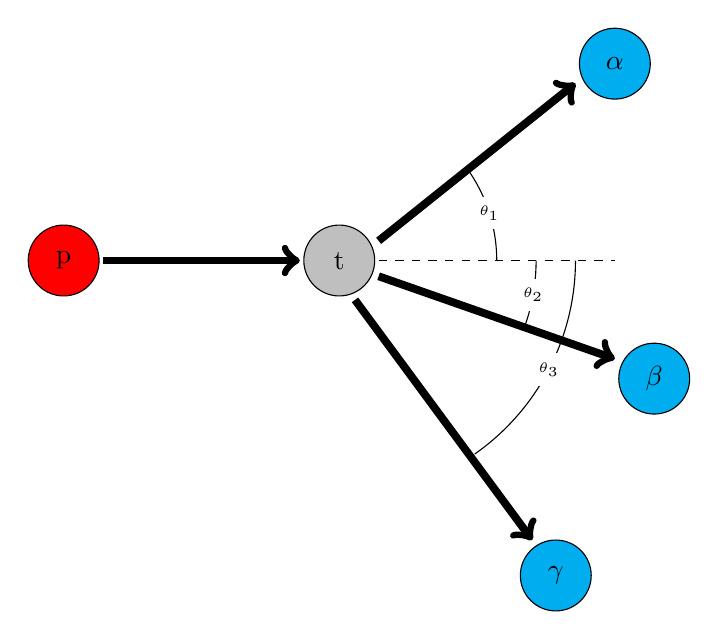
\begin{tikzpicture}
    \node[circle, draw, fill=red, minimum size = 0.9cm] (c) at (-3.5,0){p}; 
    \draw [-to, line width=1mm] (-3,0) -- (-0.5,0);
    \node[circle, draw, fill=lightgray, minimum size = 0.9cm] (c) at (0,0){t}; 
    \node[circle, draw, fill=cyan, minimum size = 0.9cm] (c) at (3.5, 2.5){$\alpha$}; 
    \node[circle, draw, fill=cyan, minimum size = 0.9cm] (c) at (4.0,-1.5){$\beta$}; 
    \node[circle, draw, fill=cyan, minimum size = 0.9cm] (c) at (2.75,-4.0){$\gamma$}; 
    \draw [-to, line width=1mm] (0.5,0.25) -- (3,2.25);
    \draw [-to, line width=1mm] (0.50,-0.20) -- (3.5,-1.25);
    \draw [-to, line width=1mm] (0.20,-0.50) -- (2.45,-3.55);
    \draw [dashed] (0.5,0) -- (3.5,0);
    \draw (2,0) arc [start angle=0, end angle=35, x radius=2cm, y radius =2cm] node[midway,fill=white] {{\tiny $\theta_1$}};
    \draw (2.5,0) arc [start angle=0, end angle=-20, x radius=2.5cm, y radius =2.5cm] node[midway,fill=white] {{\tiny $\theta_2$}};
    \draw (3,0) arc [start angle=0, end angle=-55, x radius=3cm, y radius =3cm] node[midway,fill=white] {{\tiny $\theta_3$}};
  \end{tikzpicture}
\end{document}